%!TEX root = notes.tex

\chapter{Numerical Approximation for Unconstrained Optimization}\label{chapter:nonlinearoptimization}
Although technically any characterization result finds the exact value of the extrema of a function, computationally this is hardly feasible (specially for functions of very high dimension).  See the following session based on problem \ref{problem:tricky} for an example, where we try to find the critical points of the function $f(x,y,z)=e^{x^2+y^2+z^2}-x^4-y^y-z^6$ symbolically in Python with the \texttt{sympy} libraries:

% framesep=2mm,
% baselinestretch=1.2,
\begin{minted}[frame=single, fontsize=\footnotesize, linenos ]{python}
# Importing necessary symbols/libraries/functions
from sympy.abc import x,y,z
from sympy import Matrix, solve, exp
from sympy.tensor.array import derive_by_array

# Description of f, computation of its gradient and Hessian
f = exp(x**2 + y**2 + z**2) - x**4 -y**6 - z**6
gradient = derive_by_array(f, [x,y,z])
hessian  = Matrix([derive_by_array(gradient, a) for a in [x,y,z]])
\end{minted}
While the correct expressions for $\gradient{f}$ and $\Hess{f}$ are quickly computed, trying to find critical points results in an error:
\begin{minted}[frame=single,fontsize=\footnotesize, linenos, firstnumber=10,mathescape]{python}
# Search of critical points by solving $\gradient{f}=0$
solve(gradient)
\end{minted}

\begin{minted}[frame=lines,fontsize=\footnotesize]{python}
NotImplementedError: could not solve 
4*x**2*sqrt(-log(exp(x**2)/(2*x**2))) - 6*(-log(exp(x**2)/(2*x**2)))**(5/2)
\end{minted}

Too complex a task to be performed symbolically, although the obvious answer is $(0,0,0)$.  A better way to approach this is by trying to approximate this minimum using the structure of the graph of $f$.  In these notes we are going to explore several strategies to accomplish this task, based on the concept of \emph{iterative methods for finding zeros of real-valued functions}.

\begin{example}[The Newton-Raphson method]
In order to find a many correct decimal places of $\sqrt{2}$, we allow a computer to find better and better approximations of the solution of the equation $f(x)=x^2-2$.  We start with a decent guess, say $x_0=3$.  We construct a sequence $\{ x_n \}_{n\in\field{N}}$ that converges to $\sqrt{2}$ as follows:
\begin{enumerate}
\item Find the tangent line to the graph of $f$ at $x_0$, 
\begin{equation*}
y-f(x_0)=f'(x_0)(x-x_0)
\end{equation*}
\item Provided this line is not horizontal ($f'(x_0)\neq 0$), report the intersection of this line with the $x$--axis.  Call this intersection $x_1$
\begin{equation*}
x_1=x_0-\frac{f(x_0)}{f'(x_0)}
\end{equation*}
\item Repeat this process, to get the sequence 
\begin{equation*}
x_{n+1} = x_n- \frac{f(x_n)}{f'(x_n)}
\end{equation*}
\end{enumerate}
\begin{figure}[ht!]
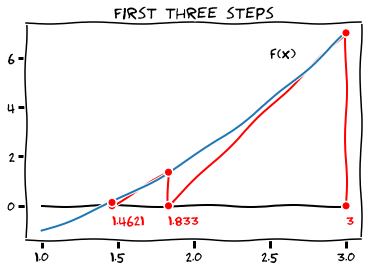
\includegraphics[width=0.65\linewidth]{newton1.png}
\caption{Newton-Raphson iterative method}
\label{figure:Newton-Raphson}
\end{figure}
Note the result of applying this process a few times:

\begin{table}[ht!]
\begin{tabular}{|c|c|r|} \hline 
$n$ & $x_n$ & $f(x_n)$ \\ \hline \hline 
$0$ & $3.000000000000000$ & $7.0000E+00$ \\ \hline 
$1$ & $1.833333333333333$ & $1.3611E+00$ \\ \hline 
$2$ & $1.462121212121212$ & $1.3780E-01$ \\ \hline 
$3$ & $1.414998429894803$ & $2.2206E-03$ \\ \hline 
$4$ & $1.414213780047198$ & $6.1568E-07$ \\ \hline 
$5$ & $1.414213562373112$ & $4.7518E-14$ \\ \hline 
$6$ & $1.414213562373095$ & $-4.4409E-16$ \\ \hline 
$7$ & $1.414213562373095$ & $4.4409E-16$ \\ \hline 
\end{tabular}
\caption{By the sixth step, the solution has already converged to a value of $\sqrt{2}$ with an accuracy of 15 digits.}
\label{table:Newton-Raphson}
\end{table}
\end{example}

Let's proceed to 
